\documentclass[12pt]{article}

\usepackage[utf8]{inputenc}%encodage des caractères
\usepackage{blindtext}
\usepackage[T1]{fontenc}%encodage de la police
\usepackage[french]{babel}%langue française
\usepackage{amsmath}
\usepackage{graphicx}
\usepackage[linesnumbered,ruled,french,onelanguage]{algorithm2e}
\usepackage{listings}
\usepackage{color}

\usepackage{url}
\usepackage{sectsty}
\usepackage{xcolor}

\usepackage{titling}%ajout de texte sur et sous le titre

%lien sans bordure
\usepackage[hypertexnames=false, pdftex]{hyperref}
\hypersetup{ colorlinks = true, linkcolor = black, urlcolor = red, citecolor = blue }

\definecolor{color_section}{RGB}{145,7,7}
\definecolor{color_subsection}{RGB}{180,70,70}
\sectionfont{\color{color_section}\underline}
\subsectionfont{\color{color_subsection}\underline \small}


\title{\hrulefill \vspace{15pt} \\ \huge \textbf{Projet de jeu de Taquin} \\ \vspace{20pt} \hrulefill  \small \textit{Complément de POO\hrulefill \vspace{40pt}}}

\author{ Marguerite Bauchez 21803320 \and Olivier Cocquerez 21803239  \and Paul Lebranchu 21403460 \and Raphaelle Lemaire 21802756  }

\date{}	
	

\begin{document}
	
	
	
\begin{titlepage}

     \renewcommand{\maketitlehooka}{
     

     \begin{flushright} \today \end{flushright}
     
     
\includegraphics[scale=1]{images/logo.png}
     
     \vspace{65pt}}
	
	
	\renewcommand{\maketitlehookd}{
	\vspace{65pt}
		
	\begin{flushright} L2 informatique \\ Groupe 3A \\ 2019-2020
	\end{flushright}
	}
     
	\maketitle
	
	\setcounter{page}{0}
\end{titlepage}


\newpage
\tableofcontents
\setcounter{page}{0}
\newpage

\section*{Introduction}
\addcontentsline{toc}{section}{Introduction}%permet d'ajouter une section non numéroter à table des matière

	Un jeu de Taquin est un jeu de puzzle à glissière, lorsque l'on clique sur une case accolée à la case vide, cette case prend la place de la case vide. En suivant ce fonctionnement, le joueur doit recréer l'image du puzzle.
	Afin de réaliser ce jeu, nous avons utiliser le langage de programmation objet Java et fait un dépôt sur SVN pour pouvoir travailler même à distance. Ce jeu sera aussi jouable dans le terminale de commande. 


	Le but de ce devoir est de réaliser une application de jeu, dotée d'une interface graphique, (mais pouvant être utilisé sans l'interface graphique) qui consiste en un puzzle à glissière.
Le joueur peut faire glisser l'un des éléments contigus à la case vide vers cette dernière (l'élément du haut, du bas, de gauche ou de droite). À tout moment, il y a donc 2, 3 ou 4 éléments déplaçables. 
Dans la partie modèle de cette application, le puzzle sera constitué de chiffres en ordre croissant sous la forme suivante (en configuration 3x3) : 
Ce sera notamment le cas dans une utilisation en ligne de commande, vu qu'il n'est pas possible d'afficher d'image dans ce contexte. 
Dans le mode de jeu version graphique, lorsque nous passerons la souris sur un élément cliquable, celui-ci sera mise en évidence(changement couleur de l'identifiant) pour indiquer au joueur qu'il pourra déplacer la case vide à cet endroit. Il sera également possible de jouer au clavier: après avoir appuyer sur la cellule vide(case 0), il sera possible de déplacer cette cellule à l'aide des flèches du clavier.
	
\vspace{10pt}

\section{Présentations}
\subsection{Model}
	La partie Model du code du jeu de Taquin est présenté dans le package Taquin. 
Elle permet de mélanger le taquin en faisant une suite de coup aléatoire, ce qui permet au jeu d'être toujours réalisable.
Ensuite, le joueur peut entrer un coup et la machine vérifie si ce coup est valide, c'est à dire, si la case que le joueur veut bouger et belle est bien accolé à la case vide.
Ainsi, le Model permet au joueur de jouer au jeu de Taquin dans le terminal et, elle sert de base au jeu de taquin au quel nous pouvons jouer de part l'interface graphique (ou vue).

\subsection{Controleur}
	La partie controleur est la partie du code qui permet au joueur d'interagir avec l'interface graphique ( ou vue). 
Lorsqu'une case est jouable, trois évènements sont ajoutés dessus: un évènements changeant l'apparence de la case quand la souris entre dedans et un autre qui réinitialise la case lorsque la souris sort, le troisième évènement permet d'intervertir cette case avec la case vide lorsque l'on clique dessus. Lorsque l'on clique sur la cellule vide, le jeu passe en mode clavier: on ajoute des évènement au touche du clavier gérant le mouvement (flèche directionnels) et lorsque le mouvement est jouable, il est effectué. Cette partie est géré par le package InterfaceGraphique.

\subsection{Vue}
	La partie vue du jeu de taquin permet d'avoir une version visuel du jeu: une image découpé en plusieurs morceaux(cases du jeu) avec un identifiant dessus. Cette partie du code est géré par le package InterfaceGraphique: ce package créé l'ensemble des boutons et des cases du jeu, il gère également la création d'un cadre de jeu. Le package créé un tableau de jeu déjà mélanger pour que le joueur puisse jouer dès le lancement de l'application. 

\vspace{10pt}

\section{Organisation du projet}

\subsection{Répartition des taches}
pour la répartition des taches, nous avons dans un premier temps diviser notre groupe en deux équipes: Olivier et Raphaëlle s’occupaient de la partie Model du jeu et Paul et Margueritte se chargeaient de la partie Vue. Une fois ces deux parties terminés, il restait à s’occuper du Controleur: cette partie a été géré en équipe malgré certaines difficultés de communication dû aux mesures de confinement.

\subsection{Gestion du projet}
Pour réaliser notre projet, nous avons utilisé différents outils:
\begin{itemize}
	\item svn :nous à permis partager les documents entre nous et faciliter le travail de groupe malgrès la distance.
	\item atom/eclipse/sublimTexte/geany: on était utiles à l'écriture du code.
	\item script .sh et archive .jar : Joue le rôle de fichier, leur façon d'être utilisé est détaillée dans le README.txt.
	\item discord/messenger : nous permettant de communiquer entre nous en dehors des cours et durant le confinement 
	\item Oracle/le cours :nous ont été utiles afin d'avoir les informations nécessaires à la bonne réalisation du projet (les sources se trouvent dans les références)
\end{itemize}

\vspace{10pt}

\section{Architecture du projet}

\subsection{Diagramme de classe/module}

Pour notre projet, nous avons réaliser trois packages: Taquin qui gère la partie modèle, InterfaceGraphique qui gère la vue et le contrôleur et Util qui permet de faire le lien entre la vue et le modèle. relié de la façon suivante:


\begin{center}
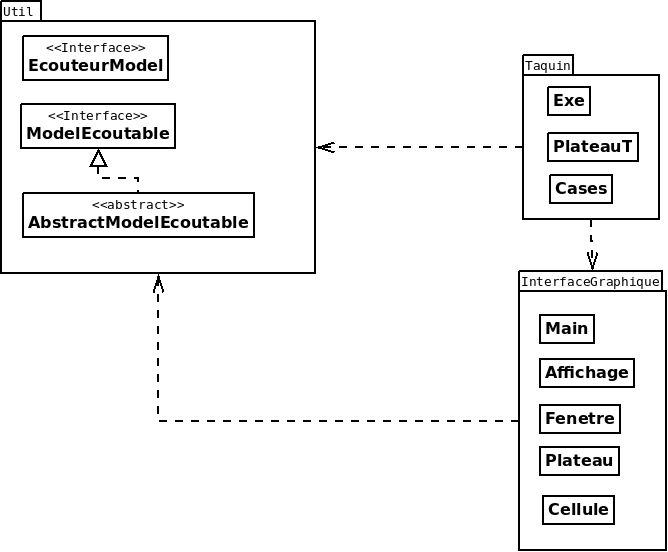
\includegraphics[scale=0.3]{images/ClasseGeneral.png}
\end{center}


Nous voyons que le package Taquin dépend du package Util et que le package InterfaceGraphique dépend à la fois de taquin et Util.

Nous allons maintenant étudier les packages de façon indépendante en commençant par le package taquin.


\begin{center}
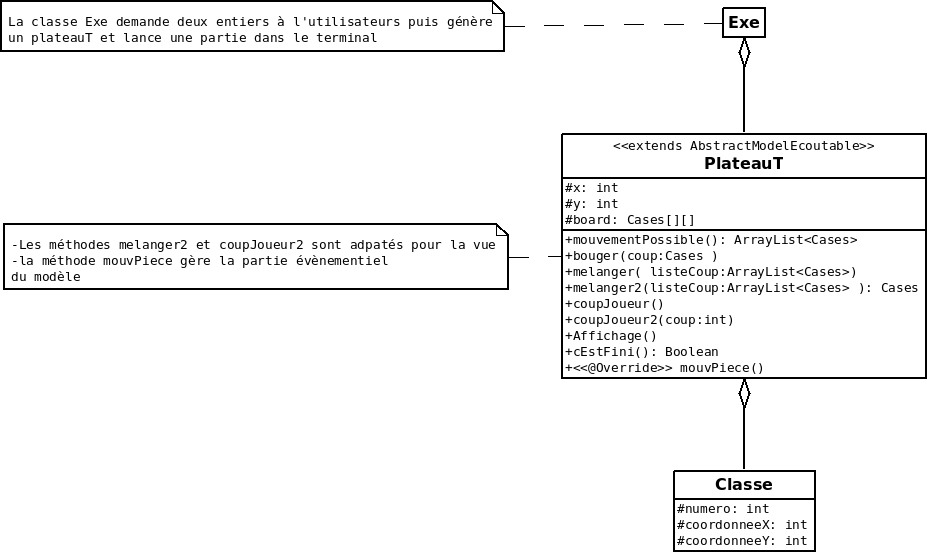
\includegraphics[scale=0.3]{images/Taquin.png}
\end{center}


Ce package gère la partie modèle du projet: la classe Cases permet de créé des cases de jeu en leur attribuant des coordonnées et un numéro, la classe PlateauT créé un plateau de jeu dans le terminal en créant un tableau à double entrée contenant les Cases du jeu et la classe Exe lance une partie de jeu dans le terminal après que l'utilisateur ait entré deux entiers définissant le nombre de lignes et de colonnes du plateau. Exe prend ces deux entiers et créé un PlateauT, il mélange ensuite les pièces de ce plateau à l'aide de la fonction mélanger avant de lancer une boucle while qui ne s’arrêtera que lorsque le taquin sera complété (c'est à dire lorsque la fonction cEstFini() renverra true).


\begin{center}
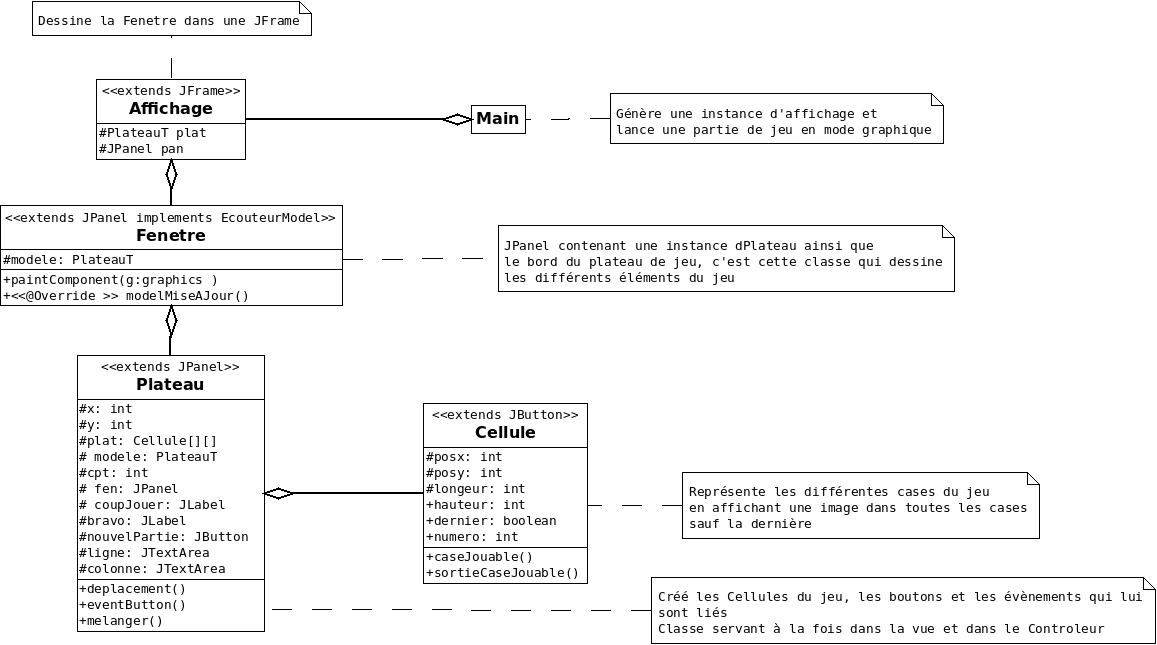
\includegraphics[scale=0.3]{images/InterfaceGraphique.png}
\end{center}


Le package Interface Graphique gère tout ce qui concerne la partie vue et contrôleur du programme. La classe Cellule est un équivalant de la classe Cases mais pour la partie graphique: elle créé des boutons qui correspondront aux cases du jeu et y ajoute une image de fond ainsi qu'un numéro. La classe Plateau créé autant de Cellule qu'il y a de cases de jeu et y associe des évènements: lorsque l'on clique sur la case 0, cela nous permet de la déplacer à l'aide du clavier et lorsque l'on passe la souris sur une cellule qui peut se déplacer, son numéro devient vert: cela veut dire qu'on peut cliquer dessus pour la déplacer. Tout ces événements ne sont possibles que lorsque la méthode cEstFini du PlateauT instancié dans cette classe renvoie faux. La classe génère également un bouton permettant de lancer une nouvelle partie et un compteur de coup. La classe Fenetre a pour rôle de dessiner l'ensemble des éléments de la classe Plateau ainsi qu'une bordure pour le plateau de jeu. La classe Affichage génère une fenêtre sur notre écran où sera afficher le contenu de la classe Fenetre et la classe Main permet de lancer une partie en mode graphique.


\begin{center}
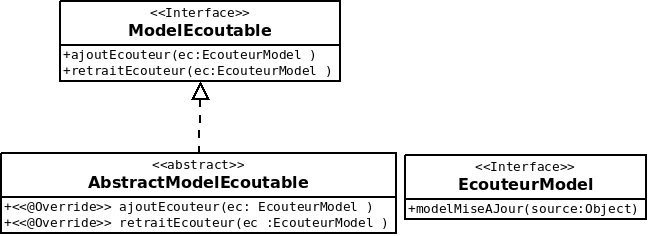
\includegraphics[scale=0.3]{images/Util.png}
\end{center}


le package Util ne contient que des interfaces et des classes abstraites. Ce sont sont ces Interfaces et cette classe abstraites qui permettent de rendre le modèle écoutables et qui rajoutes des "écouteurs" à la vue/contrôleur. 

\subsection{Cas d'utilisation}
Notre application a deux cas mode de jeu possibles:
\begin{itemize}
\item un mode console qui ne fais appel qu'au  model: il créé une instance de plateauT est demande au joueur de choisir ces coups parmi une liste de coup en rentrant son index dans la console. Le jeu dur temps que la fonction cEstFini() ne renvoie pas true. Voici une illustration d'une partie en début de jeu et en fin de jeu:



\begin{center}
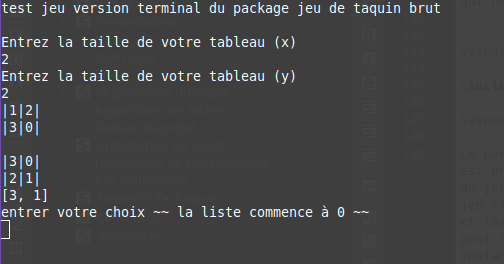
\includegraphics[scale=0.23]{images/CaptureGraphDeb.png}
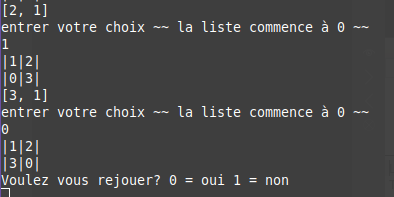
\includegraphics[scale=0.31]{images/captureGraphFin.png}
\end{center}

\item un mode graphique faisant appel à la vue/controleur et au modèle: ce mode de jeu continue tant que la méthode cEstFini du model du jeu ne renvoie pas true.


\begin{center}
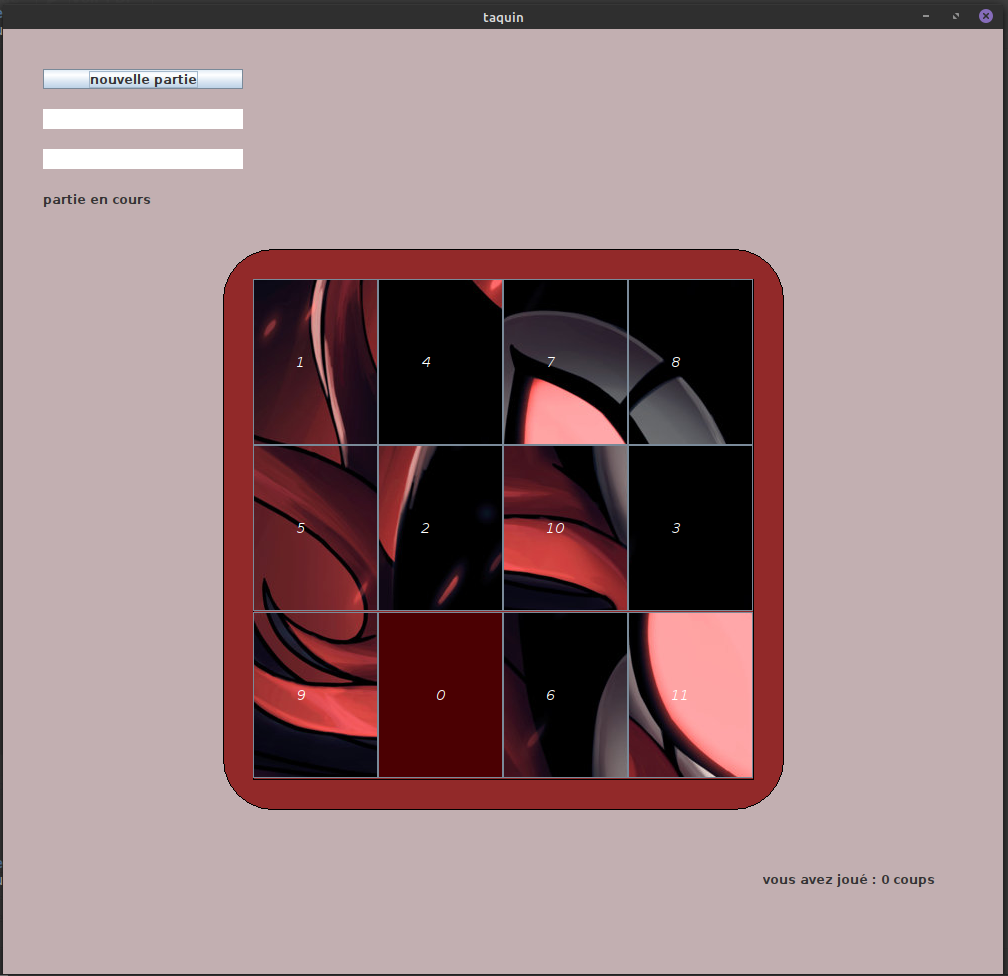
\includegraphics[scale=0.15]{images/Graph.png}
\end{center}

\end{itemize}
\vspace{10pt}

\section{Éléments Technique}
Notre codage du jeu de taquin est basé sur le paterne MVC avec un model, une vue et un controleur, ce qui le rend jouable dans un terminal et avec la souris et les touches du clavier.
Pour la partie Model donc, les éléments déplaçable du jeu, sont des case. Ces cases sont crées par la classe éponyme dans la quelle on rentre les coordonnées de la case et un numéro qui va permettre de savoir si le puzzle et résolu ou non. C'est la méthode cEstFini de la classe PlateauT qui vas vérifier si toute les cases sont au bon endroit. Dans cette classe certaine méthode sont utilisée pour le mouvement des pièces dans le terminal d'autre sont appelée dans la Vue. Ainsi, pour que nous puissions jouer, il y a la méthode mélanger qui va appliquer un certain nombre de fois la méthode coup joueur. La méthode coupJoueur permet quand à elle d'effectuer le mouvement de pièce désiré par l'utilisateur. Cette classe donne aussi la possibilité de savoir si le mouvement est possible, à l'aide d'une méthode qui récupère tout les coup possible. Ainsi, si le coup qu veux faire le joueur est invalide, il ne sera pas dans la liste et rien ne se passera.
Dans la partie vue, les pièces sont crée dans la classe cellule, dans la quelle nous rentrons une abscisse, une ordonnée ainsi que deux valeur pour la taille de la pièce, un numéro et un booléen valant True si la pièce est dernière dans le tableau. Quand on passe sur une pièce jouable sa couleur change grâce à la méthode caseJouable. La classe Plateau permet de créer le plateau de jeu pour l'affichage à l'écran. Dans cette classe la méthode deplacement permet à l'utilisateur de bouger les pièces en cliquant dessus ou avec les flèches du clavier. Elle vérifie donc sur quoi appuis l'utilisateur. La méthode eventBouton quand à elle permet de pouvoir rejouer ou créer une nouvelle partie. La classe Fenetre permet au joueur de voir le jeu et ainsi de pouvoir avoir un visuel plus joli que dans un terminal, avec en plus une image à recréer.
La partie vue et la partie Model sont liées entre elle grâce au constructeur qui met à jour le tableau par exemple.
\vspace{10pt}


\section*{Conclusion}
\addcontentsline{toc}{section}{Conclusion}

Ainsi, nous avons pu créer un jeu de taquin jouable dans le terminal avec à la place des cases, des numéros il faut donc, en intervertissant la case 0 avec une autre case acollé résoudre le puzzle. Il est aussi jouable dans une fenêtre graphique en cliquant sur les pièces de jeu qui quand on passe dessus avec la souris change de couleur et d'écriture permettant au joueur de savoir si sont coup est valide ou non. Il reste malheureusement quelque problème par exemple, nous somme obligé de cliquer sur la case vide afin de pouvoir jouer avec le clavier, de plus, nous ne gérons pas l'erreur faisant que, si l'on entre une lettre dans les zones de textes en dessous du bouton nouvelle partie, le programme affichera une erreur.

\section*{Références}
\addcontentsline{toc}{section}{Références}

\begin{itemize}
\item cours : \url{https://ecampus.unicaen.fr/course/view.php?id=14886}
\item oracle (page d'accueil): \url{https://docs.oracle.com/javase/8/docs/api/}
\item lien image du jeu: \url{https://open.spotify.com/album/3qbcMEDN44a6vdxm12FkSM}
\end{itemize}

\end{document}